\documentclass[11pt,a4paper]{article}
\usepackage[hyperref]{acl2017}
\usepackage{times}
\usepackage{latexsym}
\usepackage{tipa}
\usepackage{url}
\usepackage{booktabs}
\usepackage[utf8]{inputenc}
\usepackage{amsmath}
\usepackage{amsfonts}
\usepackage{graphicx}
\usepackage{natbib}
\usepackage{breqn}
\usepackage{todonotes}
\usepackage{arydshln}
\usepackage{enumitem}
\setlist{nolistsep}

\aclfinalcopy

\title{Encoding of phonology in a recurrent neural model of grounded speech} 

\author{
  Afra Alishahi\\
  Tilburg University\\
  {\tt a.alishahi@uvt.nl}
  \And Marie Barking\\
  Tilburg University\\
  {\tt m.barking@uvt.nl}
 \And Grzegorz Chrupała\\
  Tilburg University\\
  {\tt g.chrupala@uvt.nl}}

\date{}

\begin{document}
\maketitle

\begin{abstract}
  We study the representation and encoding of phonemes in a recurrent
  neural network model of grounded speech. We use a model which
  processes images and their spoken descriptions, and projects the
  visual and auditory representations into the same semantic space. We
  perform a number of analyses on how information about individual
  phonemes is encoded in the MFCC features extracted from the speech
  signal, and the activations of the layers of the model. Via
  experiments with phoneme decoding and phoneme discrimination we show
  that phoneme representations are most salient in the lower layers of
  the model, where low-level signals are processed at a fine-grained
  level, although a large amount of phonological information is retain at
  the top recurrent layer. We further find out that the
  attention mechanism following the top recurrent layer significantly
  attenuates encoding of phonology and makes the utterance embeddings
  much more invariant to synonymy. Moreover, a hierarchical clustering
  of phoneme representations learned by the network shows an
  organizational structure of phonemes similar to those proposed in
  linguistics.
\end{abstract}


\section{Introduction}
\label{sec:intro}

Spoken language is a universal human means of communication. As such,
its acquisition and representation in the brain is an
essential topic in the study of the cognition of our species.
In the field of neuroscience there has been a long-standing interest
in the understanding of neural representations of linguistic input in
human brains, most commonly via the analysis of neuro-imaging data of
participants exposed to simplified, highly controlled inputs. More recently, 
naturalistic data has been used and patterns in the brain have been correlated with 
patterns in the input
\citep[e.g.][]{wehbe2014simultaneously,khalighinejad2017dynamic}. 

This type of approach is relevant also when the goal is the understanding
of the dynamics in complex neural network models of speech understanding. 
Firstly because similar techniques are often applicable, but more importantly 
because the knowledge of how the workings of artificial and biological neural
networks are similar or different is valuable for the general enterprise
of cognitive science.

Recent studies have implemented models which learn to understand
speech in a weakly and indirectly supervised fashion from correlated
audio and visual signal:
\citet{harwath2016unsupervised,harwath2017learning,chrupala2017representations}. This
is a departure from typical Automatic Speech Recognition (ASR) systems
which rely on large amounts of transcribed speech, and these recent
models come closer to the way humans acquire language in a grounded
setting. It is thus especially interesting to investigate to what extent the
traditional levels of linguistic analysis such as phonology,
morphology, syntax and semantics are encoded in the activations of
the hidden layers of these models. There are a small number of
studies which focus on the syntax and/or semantics in the context of
neural models of written language
\citep[e.g.][]{elman1991distributed,frank2013acquisition,Kdr2016RepresentationOL,
li2016visualizing,adi2016fine,DBLP:journals/corr/LiMJ16a,TACL972}.
% 
Taking it a step further, \citet{gelderloos2016from} and \citet{chrupala2017representations} 
investigate the levels of representations in models which learn
language from phonetic transcriptions and from the speech signal,
respectively. Neither of these tackles the representation of phonology
in any great depth. Instead they work with relatively coarse-grained
distinctions between form and meaning.

In the current work we use controlled synthetic stimuli,
as well as  alignment between the audio signal and phonetic
transcription of spoken utterances to extract phoneme 
representation vectors based on the activations on the hidden 
layers of a model of grounded speech perception. We use these 
representations to carry out analyses of the representation of phonemes 
 at a fine-grained level. In a series of experiments, we show that 
 the lower layers of the model encode accurate representations 
 of the phonemes which can be used in phoneme identification and 
 classification with high accuracy. We further investigate how the 
 phoneme inventory is organised in the activation space of the 
 model. Finally, we tackle the general issue of the representation 
 of phonological form versus meaning with a controlled task of 
 synonym discrimination.
 
Our results show that the bottom layers in the multi-layer recurrent
neural network learn invariances which enable it to encode phonemes
independently of co-articulatory context, and that they represent
 phonemic categories closely matching usual classifications from
 linguistics. Phonological form becomes harder to detect in
 higher layers of the network, which increasingly focus on
 representing meaning over form, but encoding of phonology persists 
 to a significant degree up to the top recurrent layer.

We make the data and open-source code to reproduce our results publicly
available at
\href{https://github.com/gchrupala/encoding-of-phonology}{github.com/gchrupala/encoding-of-phonology}.


\section{Related Work}
\label{sec:related}
Research on encoding of phonology has been carried out from a 
psycholinguistics as well as computational modeling perspectives. Below we review
both types of work.
\subsection{Phoneme perception}
\label{sec:phoneme-perception}
%%%%%%%%%%%%%%%%%%%%%%%%%%%%%%% Phoneme perception
Co-articulation and interspeaker variability make it impossible to
define unique acoustic patterns for each phoneme. In an early
experiment, \citet{liberman1967perception}
analyzed the acoustic properties of the /d/ sound in the two syllables
/di/ and /du/. They found that while humans easily noticed differences
between the two instances when /d/  was played in
isolation, they perceived the /d/ as being the same when 
listening to the complete syllables. This phenomenon
is often referred to as categorical perception: acoustically different stimuli 
are perceived as the same. In another experiment \citet{lisker1967} used 
the two syllables /ba/ and /pa/ which only differ in their 
{\it voice onset time} (VOT), 
%and created a intermediates between the two syllables 
%by smoothly varying VOT. Participants clearly
%identified the consonant with VOT below 25 msec 
and created a continuum moving from syllables with short VOT 
to syllables with increasingly longer VOT. Participants identified all consonants 
with VOT below 25 msec as being /b/ and all
consonant with VOT above 25 msec as being /p/. There was no grey area in which both interpretations of the sound were equally likely, which suggests that the phonemes were perceived categorically.
Supporting findings also come from discrimination experiments: when one consonant has a VOT below 25 msec and the other above, people perceive the two syllables as being different (/ba/ and /pa/ respectively), but they do not notice any differences in the acoustic signal when both syllables have a VOT below or above 25 msec (even when these sounds are physically further away from each other than two sounds that cross the 25 msec dividing line). 
%Supporting findings also come
%from discrimination experiments: while people clearly discriminate
%between /b/ and /p/ when the two acoustic forms come from both sides
%of the 25 msec dividing line, they do not notice any differences
%between acoustic forms from the same side, even when these sounds are
%closer together physically than two sounds from different sides of the
%dividing line. 

Evidence from infant speech perception studies suggests that infants
also perceive phonemes categorically  \citep{eimas1971speech}: one-
and four-month old infants were presented with multiple syllables from
the continuum of /ba/ to /pa/ sounds described above. As long as the
syllables all came from above or below the 25 msec line, the infants
showed no change in behavior (measured by their amount of sucking),
but when presented with a syllable crossing that line, the infants
reacted differently. This suggests that infants, just like adults, perceive speech sounds as belonging to discrete categories. \citet{dehaene2004common} also showed that the same neural systems are activated for both infants and adults when performing this task.
%Studies of infants show that they also perceive
%phonemes categorically  \citep{eimas1971speech}. 
%\citet{dehaene2004common} showed that
%the same neural systems are activated for phoneme discrimination in
%children and adults.  

Importantly, languages differ in their phoneme inventories; for example English distinguishes /r/ from /l/ while Japanese does not, and children have to learn which categories to use. Experimental evidence suggests that infants can discriminate both native and nonnative speech sound differences up to 8 months of age, but have difficulty discriminating acoustically similar nonnative contrasts by 10-12 months of age \citep{werker2015critical}. These findings suggest that by their first birthday, they have learned to focus only on those contrasts that are relevant for their native language and to neglect those which are not. Psycholinguistic theories assume that children learn the categories of their native language by keeping track of the frequency distribution of acoustic sounds in their input. The forms around peaks in this distribution are then perceived as being a distinct category. Recent computational models showed that infant-directed speech contains sufficiently clear peaks for such a distributional learning mechanism to succeed and also that top-down processes like semantic knowledge and visual information play a role in phonetic category learning \citep{ter2016semantics}.

%However, languages differ in their phoneme
%inventories, for example, English distinguishes /r/ from /l/ while
%Japanese does not. Experimental evidence suggests that up to 8 months
%of age, infants reliably discriminate both native and nonnative speech
%sound differences, but by 10–12 months of age, they have difficulty
%discriminating acoustically similar nonnative contrasts \citep{werker2015critical}.Psycholinguistic theories assume that
%children keep track of the frequency distribution in their input so
%that phonemes around peaks in this distribution are perceived as being
%a distinct category. Recent computational models showed that
%infant-directed speech contains sufficiently clear peaks for such a
%distributional learning mechanism to succeed and also that top-down processes
%like semantic knowledge and visual information play a role in phonetic
%category learning \citep{ter2016semantics}.

From the machine learning perspective categorical perception
corresponds to the notion of learning invariances to certain
properties of the input. With the experiments in
Section~\ref{sec:experiments} we attempt to gain some insight into this issue.

%------------------
\subsection{Computational models}
\label{sec:computational}
There is a sizeable body of work on using recurrent neural (and other)
networks to detect phonemes or phonetic features as a subcomponent of
an ASR system. 
\citet{KING2000333} train recurrent neural networks to extract
phonological features from framewise cepstral representation of speech
in the TIMIT speaker-independent
database. 
\citet{frankel2007articulatory} introduce a dynamic Bayesian network
for articulatory (phonetic) feature recognition as a component of an ASR system.
%\citet{sroka2005human} ...
\citet{Siniscalchi2013148} show that a multilayer perceptron can 
successfully classify phonological features and contribute to the
accuracy of a downstream ASR system.

\citet{mohamed2012understanding} use a Deep Belief Network (DBN) for 
acoustic modeling and phone recognition on human speech. They analyze 
the impact of the number of layers on phone recognition error rate, and 
visualize the MFCC vectors as well as the learned activation vectors 
of the hidden layers of the model. They show that the representations learned 
by the model are more speaker-invariant than the MFCC features. 

These works directly supervise  the networks to recognize phonological
information. Another supervised but multimodal approach is taken by 
\citet{sun2016speech}, which uses grounded speech for improving a 
supervised model of transcribing utterances from 
spoken description of images. We on the other hand are more interested 
in understanding how the phonological level of representation emerges 
from weak supervision via correlated signal from the visual modality.

There are some existing models which learn language representations from sensory 
input in such a weakly supervised fashion. For example \citet{Roy2002113} use 
spoken utterances paired with images of objects, and search for segments 
of speech that reliably co-occur with visual shapes. \citet{yu2004multimodal} 
use a similar approach but also include non-verbal cues such as gaze and 
gesture into the input for unsupervised learning of words and their visual 
meaning. These language learning models use rich input signals, but are 
very limited in scale and variation. 

A separate line of research has used neural networks for modeling
phonology from a (neuro)-cognitive perspective.
\citet{burgess1999memory} implement a connectionist model of the
so-called phonological loop, i.e.\ the posited working memory which
makes phonological forms available for recall
\citep{baddeley1974working}.  \citet{gasser1989networks} show that
Simple Recurrent Networks are capable of acquiring phonological
constraints such as vowel harmony or phonological alterations at
morpheme boundaries. \citet{touretzky1989computational} present a
connectionist architecture which performs multiple simultaneous insertion,
deletion, and mutation operations on sequences of phonemes. In this body of
work the input to the network is at the level of phonemes or phonetic
features, not acoustic features, and it is thus more concerned with the
rules governing phonology and does not address how representations of
phonemes arise from exposure to speech in the first place. Moreover,
the early connectionist work deals with constrained, 
toy datasets. Current neural network architectures and hardware enable us
to use much more realistic inputs with the potential to lead to
qualitatively different results.



\section{Model}
\label{sec:model}
As our model of language acquisition from grounded speech signal we
adopt the Recurrent Highway Network-based model
of \citet{chrupala2017representations}. This model has two
desirable properties: firstly, thanks to the analyses carried in 
that work, we understand roughly how the
hidden layers differ in terms of the level of linguistic
representation they encode. Secondly, the model is trained on clean
synthetic speech which makes it appropriate to use for the controlled
experiments in Section~\ref{sec:abx}.
We refer the reader to \citet{chrupala2017representations} for a
detailed description of the model architecture. Here we give a brief
overview.

The model exploits correlations between two modalities, i.e.\ speech
and vision, as a source of weak supervision for learning to understand
speech; in other words it implements language acquisition from the
speech signal grounded in visual perception.  The architecture is a
bi-modal network whose learning objective is to project spoken
utterances and images to a joint semantic space, such that
corresponding pairs $(u,i)$ (i.e.\ an utterance and the image it
describes) are close in this space, while unrelated pairs are far
away, by a margin $\alpha$:
\begin{dmath}
  \sum_{u,i} \left(\sum_{u'} \max[0, \alpha + d(u,i) - d(u',i)] +
    \sum_{i'} \max[0, \alpha + d(u,i) - d(u,i')] \right)
\end{dmath}
where $d(u,i)$ is the cosine distance between the encoded utterance $u$
and encoded image $i$.

The image encoder part of the model uses image vectors from a
pretrained object classification model, VGG-16 \citep{simonyan2014very}, and uses a linear
transform to directly project these to the joint space.
The utterance encoder takes Mel-frequency Cepstral Coefficients (MFCC)
as input, and transforms it successively according to:
\begin{equation}
  \label{eq:encode_u}
  \mathrm{enc}_u(\mathbf{u}) = \mathrm{unit}(\mathrm{Attn}(\mathrm{RHN}_{k,L} (\mathrm{Conv}_{s,d,z}(\mathbf{u}))))
\end{equation}
The first layer $\mathrm{Conv}_{s,d,z}$ is a one-dimensional
convolution of size $s$ which subsamples the input with stride $z$,
and projects it to $d$ dimensions. It is followed by
$\mathrm{RHN}_{k,L}$ which consists of $k$ residualized recurrent
layers. Specifically these are Recurrent Highway Network layers
\citep{zilly2016recurrent}, which are closely related to GRU networks,
with the crucial difference that they increase the depth of the
transform between timesteps; this is the recurrence depth $L$. The
output of the final recurrent layer is passed through an
attention-like lookback operator $\mathrm{Attn}$ which takes a
weighted average of the activations across time steps. Finally,
both utterance and image projections are L2-normalized. See
Section~\ref{sec:parameters} for details of the model configuration.


\section{Experimental data and setup}
\label{sec:experiments}
The phoneme representations in each layer are calculated as the
activations averaged over the duration of the phoneme occurrence in the
input. The average input vectors are similarly calculated as the MFCC
vectors averaged over the time course of the articulation of the
phoneme occurrence. When we need to represent a phoneme type we do so by
averaging the vectors of all its occurrences in the validation set.
\begin{table}[t]
  \centering
  \begin{tabular}{l|c}
    Vowels & \textipa{i I U u}\\
           & \textipa{e E \textschwa{} \textrhookschwa{} OI O o }
             \\
           & \textipa{aI \ae{} \textturnv{} \textscripta{}  aU }\\
    Approximants & \textipa{j \textturnr{} l w }\\
    Nasals      & \textipa{m n N } \\
    Plosives   & \textipa{p  b  t  d  k  g }\\
    Fricatives & \textipa{f v T \dh{} s z S Z h }\\
    Affricates & \textipa{\textteshlig{} \textdyoghlig{} }\\
  \end{tabular}
  \caption{Phonemes of General American English.}
  \label{tab:phoneme-list}
\end{table}
Table~\ref{tab:phoneme-list} shows the phoneme inventory we work with; this is also the inventory used by Gentle/Kaldi (see Section~\ref{sec:forced}).


\subsection{Model settings}
\label{sec:parameters}
We use the pre-trained version of the COCO~Speech model, implemented
in Theano \citep{Bastien-Theano-2012}, provided by
\citet{chrupala2017representations}.\footnote{Code, data and
  pretrained models available from \href{https://github.com/gchrupala/visually-grounded-speech}{https://github.com/gchrupala/visually-grounded-speech}.}
The details of the model configuration are as follows: convolutional
layer with length 6, size 64, stride 3, 5 Recurrent Highway Network
layers with 512 dimensions and 2 microsteps, attention Multi-Layer
Perceptron with 512 hidden units, Adam optimizer, initial learning
rate 0.0002. The 4096-dimensional image feature vectors come from the
final fully connect layer of VGG-16 \citep{simonyan2014very}
pre-trained on Imagenet \cite{ILSVRCarxiv14}, and are averages of
feature vectors for ten crops of each image.  The total number of
learnable parameters is 9,784,193. Table~\ref{tab:arch} sketches the
architecture of the utterance encoder part of the model.

\begin{table}[t]
  \centering
  \begin{tabular}{|c|}\hline
    Attention: size 512 \\\hline
    Recurrent 5: size 512 \\\hline
    Recurrent 4: size 512 \\\hline
    Recurrent 3: size 512 \\\hline
    Recurrent 2: size 512 \\\hline
    Recurrent 1: size 512 \\\hline
    Convolutional: size 64, length 6, stride 3 \\\hline\hline
    Input MFCC: size 13 \\\hline
  \end{tabular}
  \caption{COCO~Speech utterance encoder architecture.}
  \label{tab:arch}
\end{table}

\subsection{Synthetically Spoken COCO}
\label{sec:coco}
The Speech~COCO model was trained on the Synthetically Spoken COCO dataset \citep{grzegorz_chrupala_2017_400926}, which is a version of the MS~COCO dataset \citep{lin2014microsoft} where speech was synthesized for the original image descriptions, using high-quality speech synthesis provided by gTTS.\footnote{Available at \href{https://github.com/pndurette/gTTS}{https://github.com/pndurette/gTTS}.}

\subsection{Forced alignment}
\label{sec:forced}
We aligned the speech signal to the corresponding phonemic transcription with the Gentle toolkit,\footnote{Available at
  \href{https://github.com/lowerquality/gentle}{https://github.com/lowerquality/gentle}.}
which in turn is based on Kaldi \citep{Povey_ASRU2011}. It 
uses a speech recognition model for English to transcribe the input audio
signal, and then finds the optimal alignment of the transcription to
the signal. This fails for a small number of utterances, which we
remove from the data.  In the next step we extract MFCC features from
the audio signal and pass them through the COCO~Speech utterance encoder, and
record the activations for the convolutional layer as well as all the
recurrent layers. For each utterance the representations (i.e.\ MFCC
features and activations) are stored in a $t_r\times D_r$ matrix, where
$t_r$ and $D_r$ are the number of times steps and the dimensionality,
respectively, for each representation $r$. Given the alignment of each
phoneme token to the underlying audio, we then infer the slice of the
representation matrix corresponding to it.

\section{Experiments}
In this section we report on four experiments which we designed to
elucidate to what extent information about phonology is represented in
the activations of the layers of the COCO~Speech model. In
Section~\ref{sec:decoding} we quantify how easy it is to decode phoneme
identity from activations. In Section~\ref{sec:abx} we determine
phoneme discriminability in a controlled task with minimal pair
stimuli. Section~\ref{sec:organization} shows how the phoneme
inventory is organized in the activation space of the model. Finally,
in Section~\ref{sec:synonym} we tackle the general issue of the
representation of phonological form versus meaning with the controlled
task of synonym discrimination.

\subsection{Phoneme decoding}
\label{sec:decoding}
In this section we quantify to what extent phoneme identity can be
decoded from  the input MFCC features as compared to the
representations extracted from the COCO speech. As explained in 
Section~\ref{sec:forced}, we use phonemic
transcriptions aligned to the corresponding audio in order to segment
 the signal into chunks corresponding to individual phonemes.

We take a sample of 5000 utterances from the validation set of
Synthetically Spoken COCO, and extract the force-aligned
representations from the Speech COCO model.
%using the procedure described in Section~\ref{sec:forced}. 
We split this data into $\frac{2}{3}$ training and
$\frac{1}{3}$ heldout portions, and use supervised classification in
order to quantify the recoverability of phoneme identities from the
representations. Each phoneme slice is averaged over time, so that it
becomes a $D_r$-dimensional vector. For each representation we then
train $L2$-penalized logistic regression (with the fixed penalty
weight $1.0$) on the training data and measure classification error rate
on the heldout portion. 

Figure~\ref{fig:decode} shows the results. As can be seen from this plot, phoneme recoverability 
is poor for the representations based on MFCC and the convolutional layer activations, but improves markedly for 
the recurrent layers. Phonemes are easiest recovered from the activations at recurrent
layers 1 and 2, and the accuracy decreases thereafter. This suggests
that the bottom recurrent layers of the model specialize in recognizing this
type of low-level phonological information. It is notable however that
even the last recurrent layer encodes phoneme identity to a
substantial degree.

The MFCC features do much better than majority baseline (89\% error rate) but
poorly reltive to the the recurrent layers. Averaging across
phoneme durations may be hurting performance, but interestingly, the
network can overcome this and form more robust phoneme representations in 
the activation patterns.

\begin{figure}[t]
  \centering
  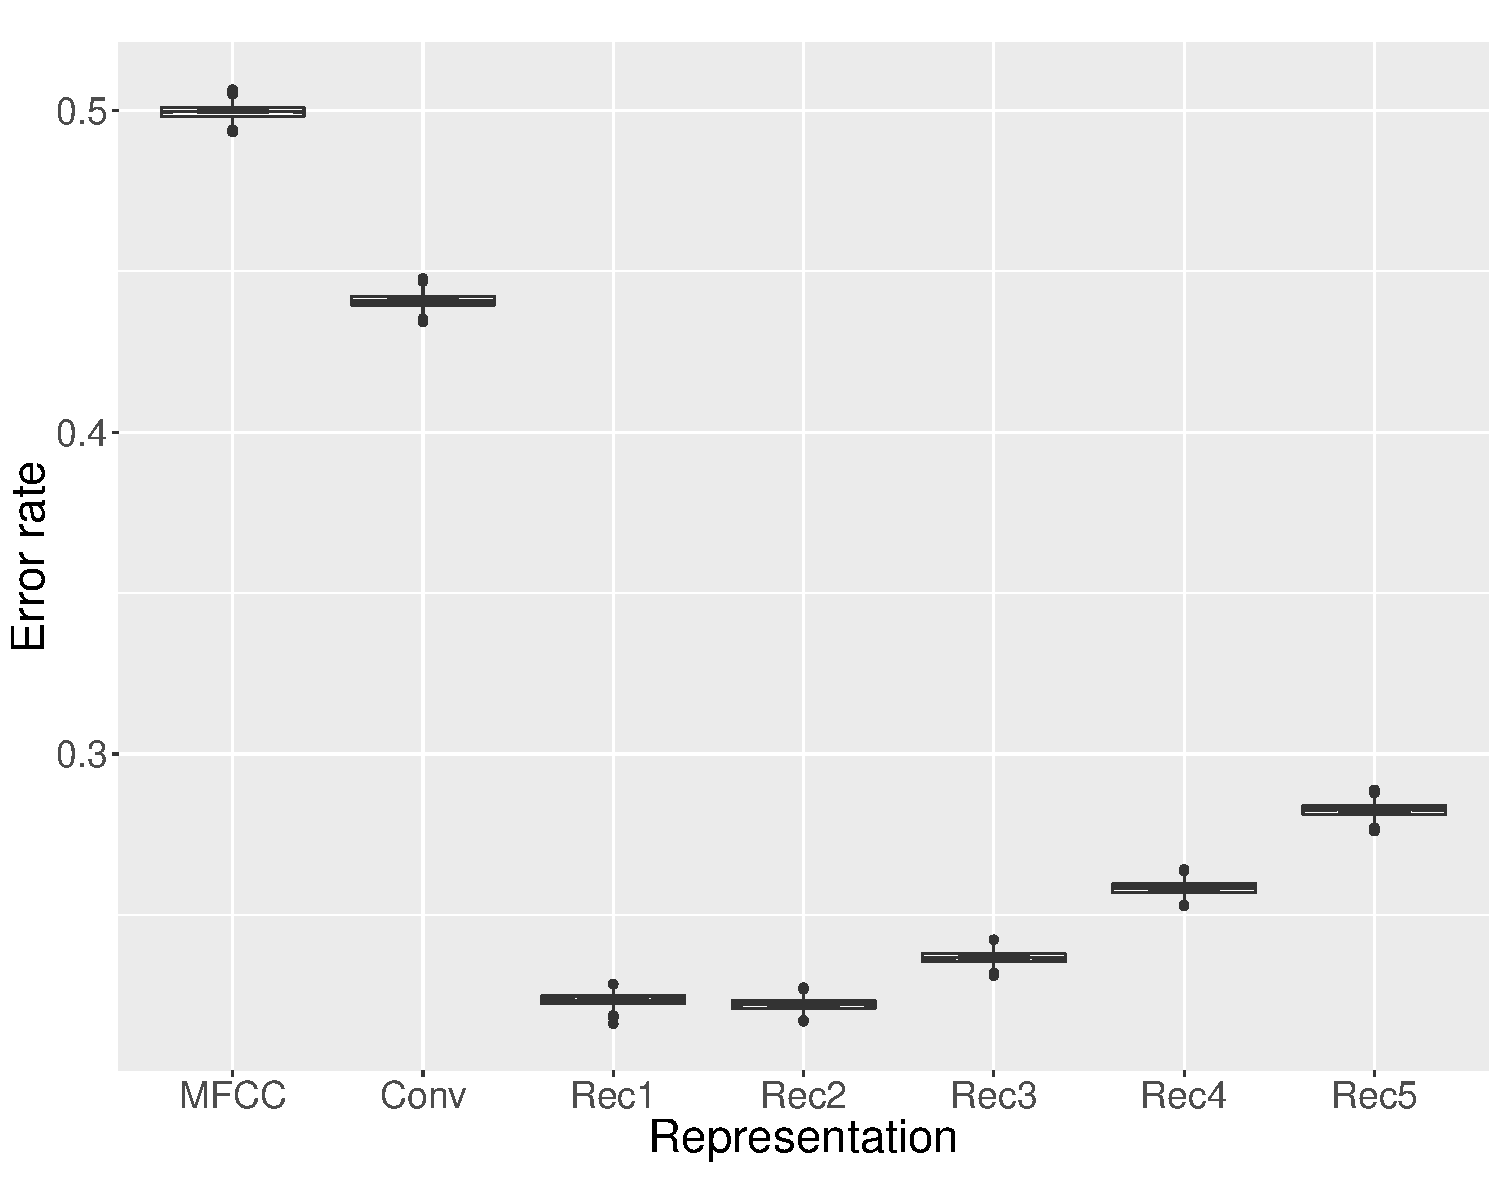
\includegraphics[scale=0.3]{figures/decode.pdf}
  \vspace{-1cm}
     \caption{Accuracy of phoneme decoding with input MFCC features
       and COCO~Speech model activations. The boxplot shows error rates
       bootstrapped with 1000 resamples.}
     \label{fig:decode}
\end{figure}
%% \begin{table}
%%   \centering
%%   \begin{tabular}{l|r}
%%     Representation  & Accuracy  \\\hline
%%     MFCC            & 0.50      \\\hdashline
%%     Convolution     & 0.56      \\
%%     Recurrent 1     & 0.77      \\
%%     Recurrent 2     & 0.78      \\
%%     Recurrent 3     & 0.76      \\
%%     Recurrent 4     & 0.74      \\
%%     Recurrent 5     & 0.72      \\
%%   \end{tabular}
%%   \caption{Accuracy of phoneme decoding with input MFCC features and
%%     COCO~Speech model activations.}
%%   \label{tab:decode}
%% \end{table}
%% ('mfcc', 0.49870657476692304)
%% ('conv', 0.55728398062466367)
%% (0, 0.77430163718120104)
%% (1, 0.77633292244657026)
%% (2, 0.76174933592597094)
%% (3, 0.74003020885779269)
%% (4, 0.71567214708588689)


\subsection{Phoneme discrimination}
\label{sec:abx}

\citet{schatz2013evaluating} propose a framework for evaluating speech features learned in an 
unsupervised setup that does not depend on phonetically labeled data. They propose a set of 
tasks called Minimal-Pair ABX tasks that allow to make linguistically precise comparisons 
between syllable pairs that only differ by one phoneme. They use variants of this task to study 
phoneme discrimination across talkers and phonetic contexts as well as talker discrimination 
across phonemes.

Here we evaluate the COCO~Speech model on the {\it Phoneme across Context} (PaC) task of 
\citet{schatz2013evaluating}. This task consists of presenting a series of equal-length tuples 
$(A, B, X)$ to the model, where $A$ and $B$ differ by one phoneme (either a vowel 
or a consonant), as do $B$ and $X$, but $A$ and $X$ are not minimal pairs.  For example, 
in the tuple ({\it be} /bi/, {\it me} /mi/, {\it my} /\textipa{maI}/),
the task is to identify which of the two syllables /bi/ or /mi/ is closer to /\textipa{maI}/.  The goal is to 
measure context invariance in phoneme discrimination by evaluating how often the model 
recognizes $X$ as the syllable closer to $B$ than to $A$.

\begin{table}
 \centering
 \caption{Accuracy of choosing the correct target in an ABX task using different 
 representations.}
 \label{tab:abx}
 \vspace{.2cm}
 \begin{tabular}{lr}
   \toprule
 { Representation} & {Accuracy} \\
 \midrule
 MFCC &  0.72 \\
 Convolutional & 0.73 \\
 Recurrent 1 &  0.83 \\
 Recurrent 2 &  0.84 \\
 Recurrent 3 &  0.80 \\
 Recurrent 4 &  0.77 \\
 Recurrent 5 &  0.75 \\
 Embeddings  &  0.67 \\
 \bottomrule
 \end{tabular}
 \end{table}


We used a list of all attested consonant-vowel (CV) syllables of American English according to 
the syllabification method described in \citet{Gorman2013}. We excluded the ones which could 
not be unambiguously represented using English spelling for input to the TTS system 
(e.g.\ /\textipa{baU}/). We then compiled a list of all possible $(A, B, X)$ tuples from this list 
where $(A,B)$ and $(B,X)$ are minimal pairs, but $(A,X)$ are not. 
This resulted in 34,288 tuples in total. For each tuple, we measure 
$\mathrm{sign}(\mathrm{dist}(A,X) - \mathrm{dist}(B,X))$, where $\mathrm{dist}(i,j)$ is the 
euclidean distance between the vector 
representations of syllables $i$ and $j$. These representations are either the audio feature 
vectors or the layer activation vectors. A positive value for a tuple means that the model has 
correctly discriminated the phonemes that are shared or different across the syllables.

Table~\ref{tab:abx} shows the discrimination accuracy in this task using various representations. 
The pattern is similar to what we observed in the phoneme identification task: best accuracy is 
achieved using representation vectors from recurrent layers 1 and 2, and it drops as we move 
further up in the model. The accuracy is lowest when final embedding features are used for this task. 




\begin{figure}[t]
  \centering
  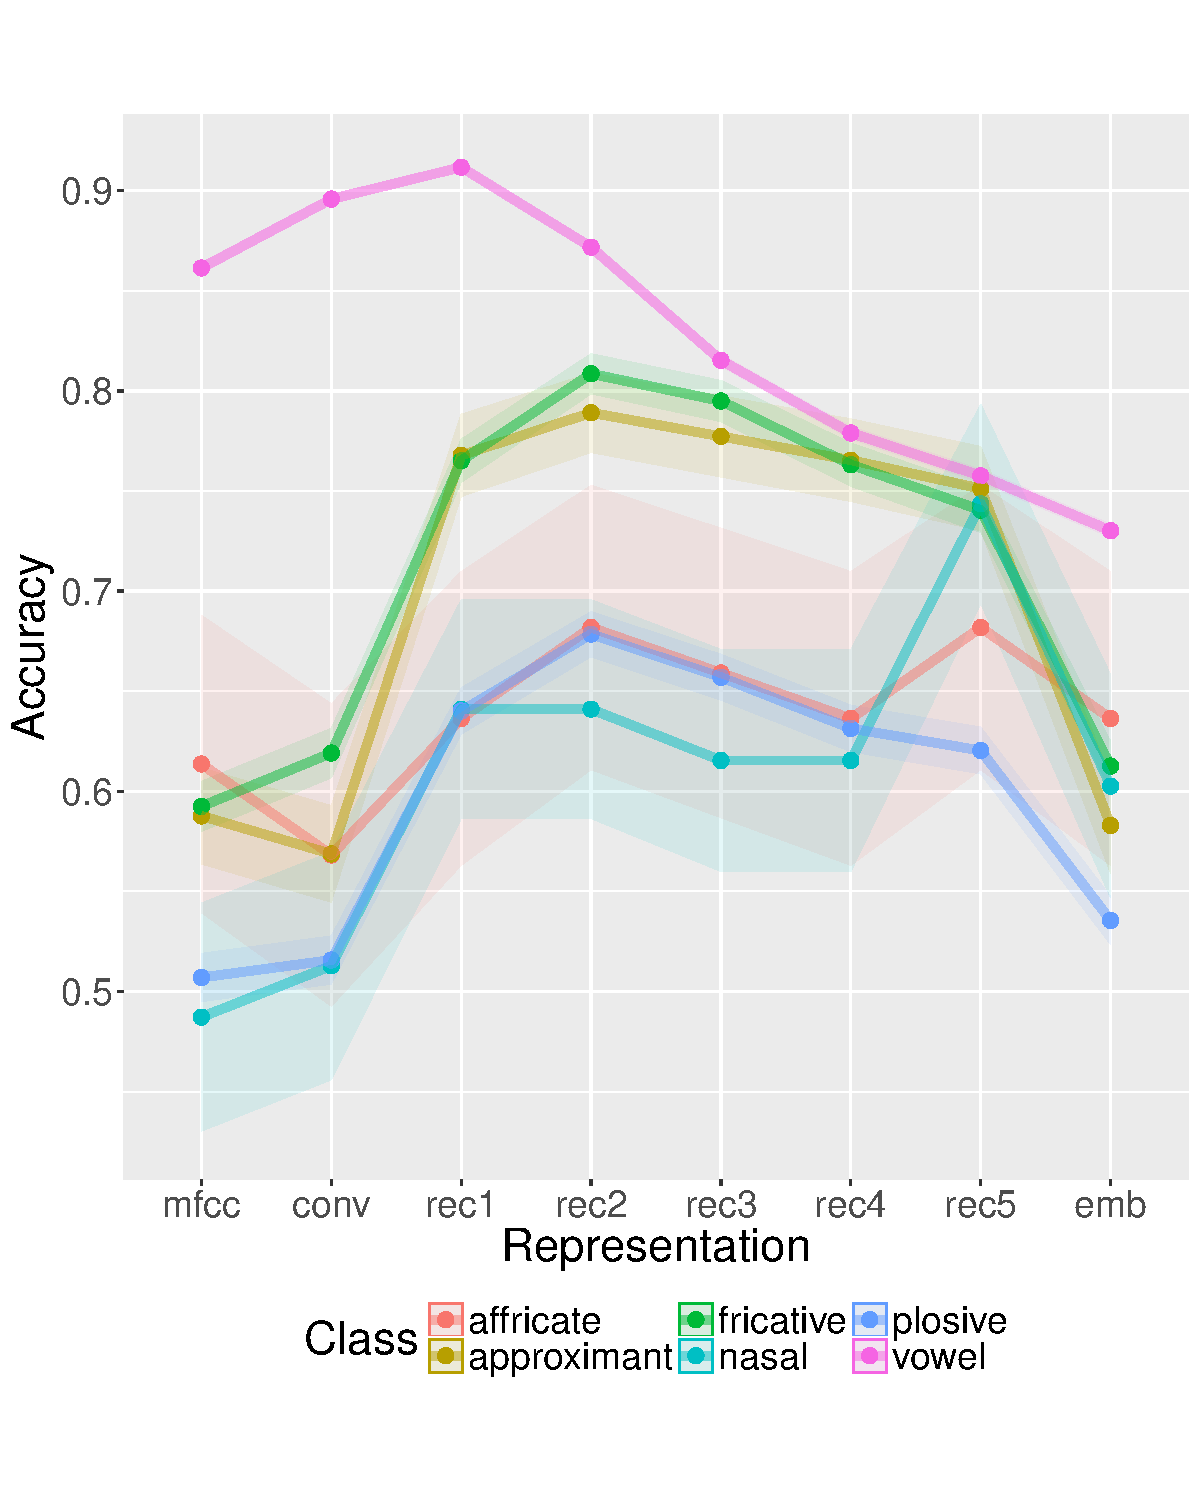
\includegraphics[scale=0.3]{figures/abx_cv_same.pdf}
  \caption{Accuracies for the ABX CV task for the cases where the target
    and the distractor belong to the same phoneme class. Shaded area
    extends $\pm1$ standard error from the mean.}
  \label{fig:abx_cv_same}
\end{figure}

However, the PaC task is most meaningful and challenging where the target and the distractor 
phonemes belong to the same phoneme class. Figure~\ref{fig:abx_cv_same} shows the 
accuracies for this subset of cases, broken down by class.
%
As can be seen, the model can discriminate between phonemes with high accuracy across all 
the layers, and the layer activations are more informative for this task than the MFCC features. 
Again, most phoneme classes seem to be represented more accurately in the lower layers (1--3), and the performance of the model in this task drops as we move towards higher hidden layers. There are also clear differences in the pattern of discriminability for the phoneme classes. The vowels are especially easy to tell apart, but accuracy on vowels drops most acutely in the higher layers. Meanwhile the accuracy on fricatives and approximants starts low, but improves rapidly and peaks around recurrent layer~2. 
The somewhat erratic pattern for nasals and affricates is most likely due to small sample size for these classes, as evident from the wide standard error. 

\subsection{Organization of phonemes}
\label{sec:organization}

In this section we take a closer look at the underlying organization
of phonemes in the model.  Our experiment is inspired by 
\citet{khalighinejad2017dynamic} who study how
the speech signal is represented in the brain at different stages of
the auditory pathway by collecting and analyzing electroencephalography 
responses from participants listening to continuous speech, and show that brain
responses to different phoneme categories turn out to be organized by
phonetic features. 
%They compared the patterns of phoneme
%similarity in the neural responses and the acoustic signals and
%demonstrated that acoustic distinctions of phonemes are reflected in
%the corresponding neural data.

%{\it I assume most of the following paragraph will move to introduction or related work, but I keep it here 
%for now to motivate the experiment. Also most of the content is copied from their paper, so we need to 
%rewrite the text.}
%
%To study how the speech signal is represented in the brain at different stages of the auditory pathway, 
%\cite{khalighinejad2017dynamic} collected electroencephalography responses to continuous speech by 
%obtaining the time-locked responses to phoneme instances (phoneme-related potential), and showed 
%that responses to different phoneme categories are organized by phonetic features. In addition, they 
%compared the patterns of phoneme similarity in the neural responses and the acoustic signals which 
%showed a repetitive appearance of acoustic distinctions of phonemes in the neural data. Their analysis 
%of the phonetic and speaker information in neural activations revealed that different time intervals jointly 
%encode the acoustic similarity of both phonetic and speaker categories. 

%Here we present a simulation of the study of \cite{khalighinejad2017dynamic} by analyzing the hidden 
%layer activations of our model in response to each phoneme in the input, and compare them to the 
%MFCC representations of these phonemes in the speech signal. 
%
%The phoneme activations in each layer, which can be thought as the model's equivalent to the phoneme-
%related potentials, and are calculated as the hidden layer activations averaged over the duration of the 
%phoneme token in the input. The average input vectors are similarly calculated as the MFCC vectors 
%averaged over the time course of the articulation of the phoneme token. Each phoneme type is 
%represented by the average input vector of all its instances in the validation set, and the average 
%activation vector of all its instances for each hidden layer in the model.
%
%%\subsubsection{Correlation with audio representations}
%
%Following \cite{khalighinejad2017dynamic}, we generated a distance matrix for every pair of phonemes 
%by calculating the euclidean distance between the phoneme pair's activation vectors for each layer 
%separately. Similarly, we calculated the distance matrix for the audio vectors of all phoneme pairs in our 
%data. We then calculated the Pearson correlations between the lower triangular part the audio distance 
%matrix and each of activation distance matrix for each layer. 
%\todo{Check that this is what we are doing.}
%>>>>>>> 5719ea4ce48084d7f0d6f9416d2c278836afbc8f



\begin{figure}[t]
  \centering
  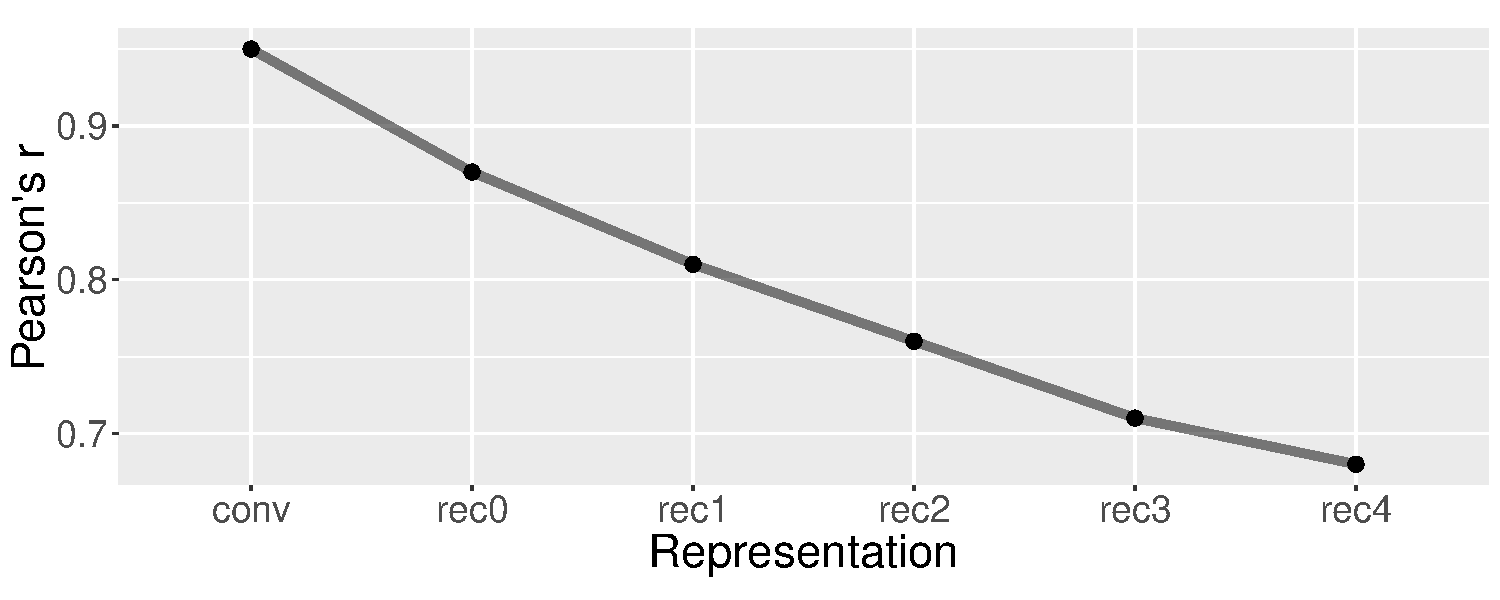
\includegraphics[scale=0.28]{figures/correlation_mfcc.pdf}
  \caption{Pearson's correlation coefficients $r$ between the distance matrix of MFCCs and distance matrices on activation vectors.}
  \label{fig:correlation}
\end{figure}


% Convolutional & 0.95 \\
% Layer 1 &  0.87 \\
% Layer 2 &  0.81 \\
% Layer 3 &  0.76 \\
% Layer 4 &  0.71 \\
% Layer 5 &  0.68 \\



We carry out an analogous experiment by analyzing the hidden layer activations of our model in 
response to each phoneme in the input. First, we generated a distance matrix 
for every pair of phonemes by calculating the Euclidean distance between the 
phoneme pair's activation vectors for each layer separately, as well as a 
distance matrix for all phoneme pairs based on their MFCC features. Similar to 
what \citet{khalighinejad2017dynamic} report,  we observe that the phoneme 
activations on all layers significantly correlate with the phoneme representations 
in the speech signal, and these correlations are strongest for 
the lower layers of the model. Figure~\ref{fig:correlation} shows the results.

%The phoneme activations in each layer, which can be thought as the model's 
%equivalent to the phoneme-
%related potentials, and are calculated as the hidden layer activations 
%averaged over the duration of the 
%phoneme token in the input. The average input vectors are similarly 
%calculated as the MFCC vectors 
%averaged over the time course of the articulation of the phoneme token. Each 
%phoneme type is 
%represented by the average input vector of all its instances in the validation 
%set, and the average 
%activation vector of all its instances for each hidden layer in the model.
%
%\subsubsection{Correlation with audio representations}


%\subsubsection{Organization of phonemes}
%\label{sec:clustering}

%\begin{table*}
%\caption{Evaluation of phoneme clusters based on audio features and layer 
%activations.}
%\label{tab:clustering}
%\begin{center}
%\begin{tabular}{c|c|c|c|c}
%&	{\bf Rand Index}& {\bf Homogeneity} & {\bf Completeness} & {\bf V-
%measure} \\
%\hline
%Audio features		& 0.27		& 0.59		& 0.52		& 0.55 \\
%Activations layer 0	& 0.23		& 0.47		& 0.45		& 0.46 \\
%Activations layer 1	& 0.16		& 0.47		& 0.45		& 0.46 \\
%Activations layer 2	& 0.16		& 0.47		& 0.45		& 0.46 \\
%Activations layer 3	& 0.15		& 0.43		& 0.48		& 0.45 \\
%Activations layer 4	& 0.15		& 0.43		& 0.48		& 0.45 \\
%\hline
%\end{tabular}
%\end{center}
%\end{table*}

%phone mode: short	activation mode: avg
%
%Clustering		Rand Index	Homogeneity	Completeness	V-measure
%Audio features	        0.27		0.59		0.52		0.55
%Conv. activations	0.12		0.44		0.40		0.42
%Activations layer 0	0.23		0.47		0.45		0.46
%Activations layer 1	0.16		0.47		0.45		0.46
%Activations layer 2	0.16		0.47		0.45		0.46
%Activations layer 3	0.15		0.43		0.48		0.45
%Activations layer 4	0.15		0.43		0.48		0.45
%
%---------
%
%phone mode: long	activation mode: avg
%
%Clustering		Rand Index	Homogeneity	Completeness	V-measure
%Audio features		0.18		0.45		0.42		0.44
%Conv. activations	0.20		0.43		0.41		0.42
%Activations layer 0	0.16		0.43		0.40		0.41
%Activations layer 1	0.11		0.39		0.39		0.39
%Activations layer 2	0.11		0.40		0.38		0.39
%Activations layer 3	0.06		0.33		0.38		0.35
%Activations layer 4	0.06		0.28		0.32		0.30

%% \begin{figure*}[t]
%%   \centering
%%   \includegraphics[scale=0.37]{figures/audio.png}
%% \caption{Hierarchical clustering of phoneme audio vectors.}
%% \label{fig:cluster-audio}
%% \end{figure*}
%% \begin{figure*}[t]
%%   \centering
%%   \includegraphics[scale=0.37]{figures/activation4.png}
%% \caption{Hierarchical clustering of phoneme activation vectors on the last 
%%  hidden layer.}
%% \label{fig:cluster-l4}
%% \end{figure*}
We then performed agglomerative hierarchical clustering on phoneme type MFCC and 
activation vectors, using Euclidean distance as the distance metric and the Ward linkage criterion \citep{ward1963hierarchical}.
%We compared the class labels extracted from the clustering tree to a set of 
%manually-annotated gold-standard labels for phoneme categories. 
%Table~\ref{tab:clustering} shows the clustering results.
Figure~\ref{fig:cluster-l0} shows the clustering results for the activation vectors
on the first hidden layer. The leaf nodes are color-coded according to phoneme classes as specified in Table~\ref{tab:phoneme-list}. There is substantial degree of matching between the classes and the structure of the hierarchy, but also some mixing between rounded back vowels and voiced plosives /b/ and /g/, which share articulatory features such as lip movement or tongue position. 
\begin{figure}[ht]
  \centering
  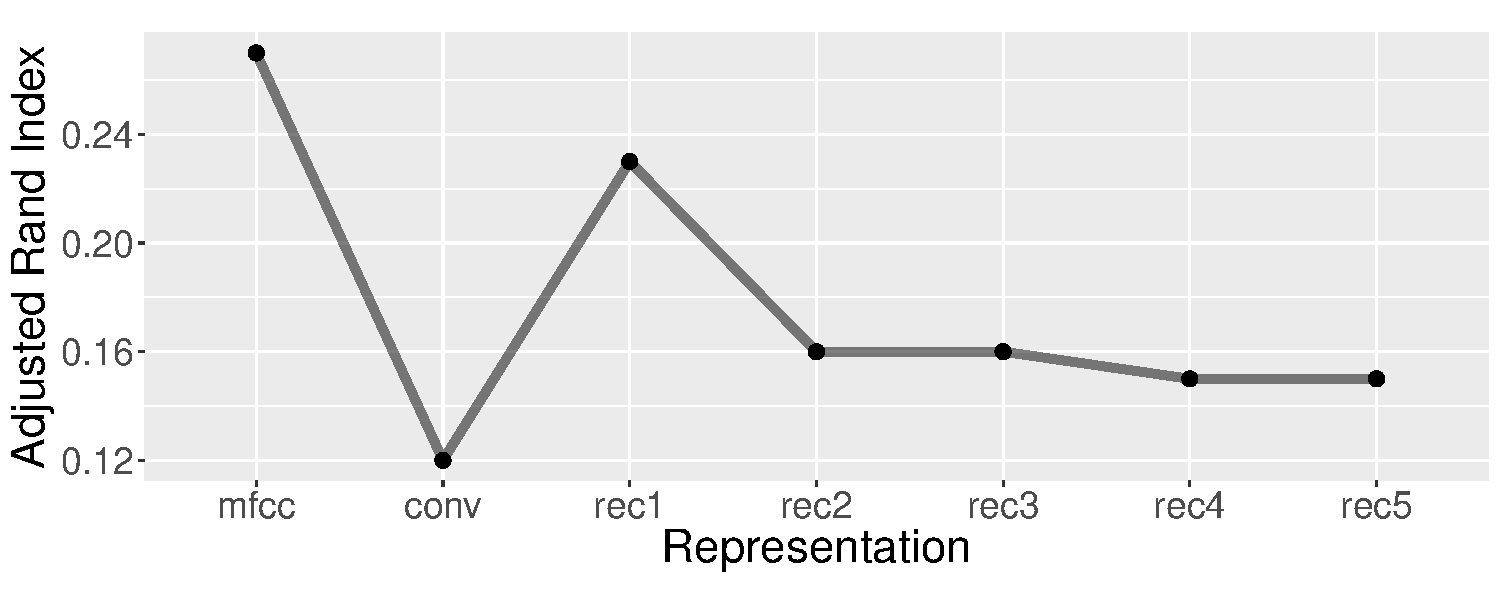
\includegraphics[scale=0.3]{figures/hier_ari.pdf}
  \caption{Adjusted Rand Index for the comparison of the phoneme type hierarchy induced from representations against phoneme classes.}
  \label{fig:hier_ari}
\end{figure}

We measured the adjusted Rand Index for the match between the
hierarchy induced from each representation against phoneme classes,
which were obtained by cutting the tree to divide the cluster into the
same number of classes as there are phoneme classes. There is a notable drop between the match from MFCC to the activation of the convolutional layer. We suspect this may be explained by the loss of information caused by averaging over phoneme instances combined with the lower temporal resolution of the activations compared to MFCC. The match improves markedly at recurrent layer~1.


\begin{figure*}[t]
  \centering
  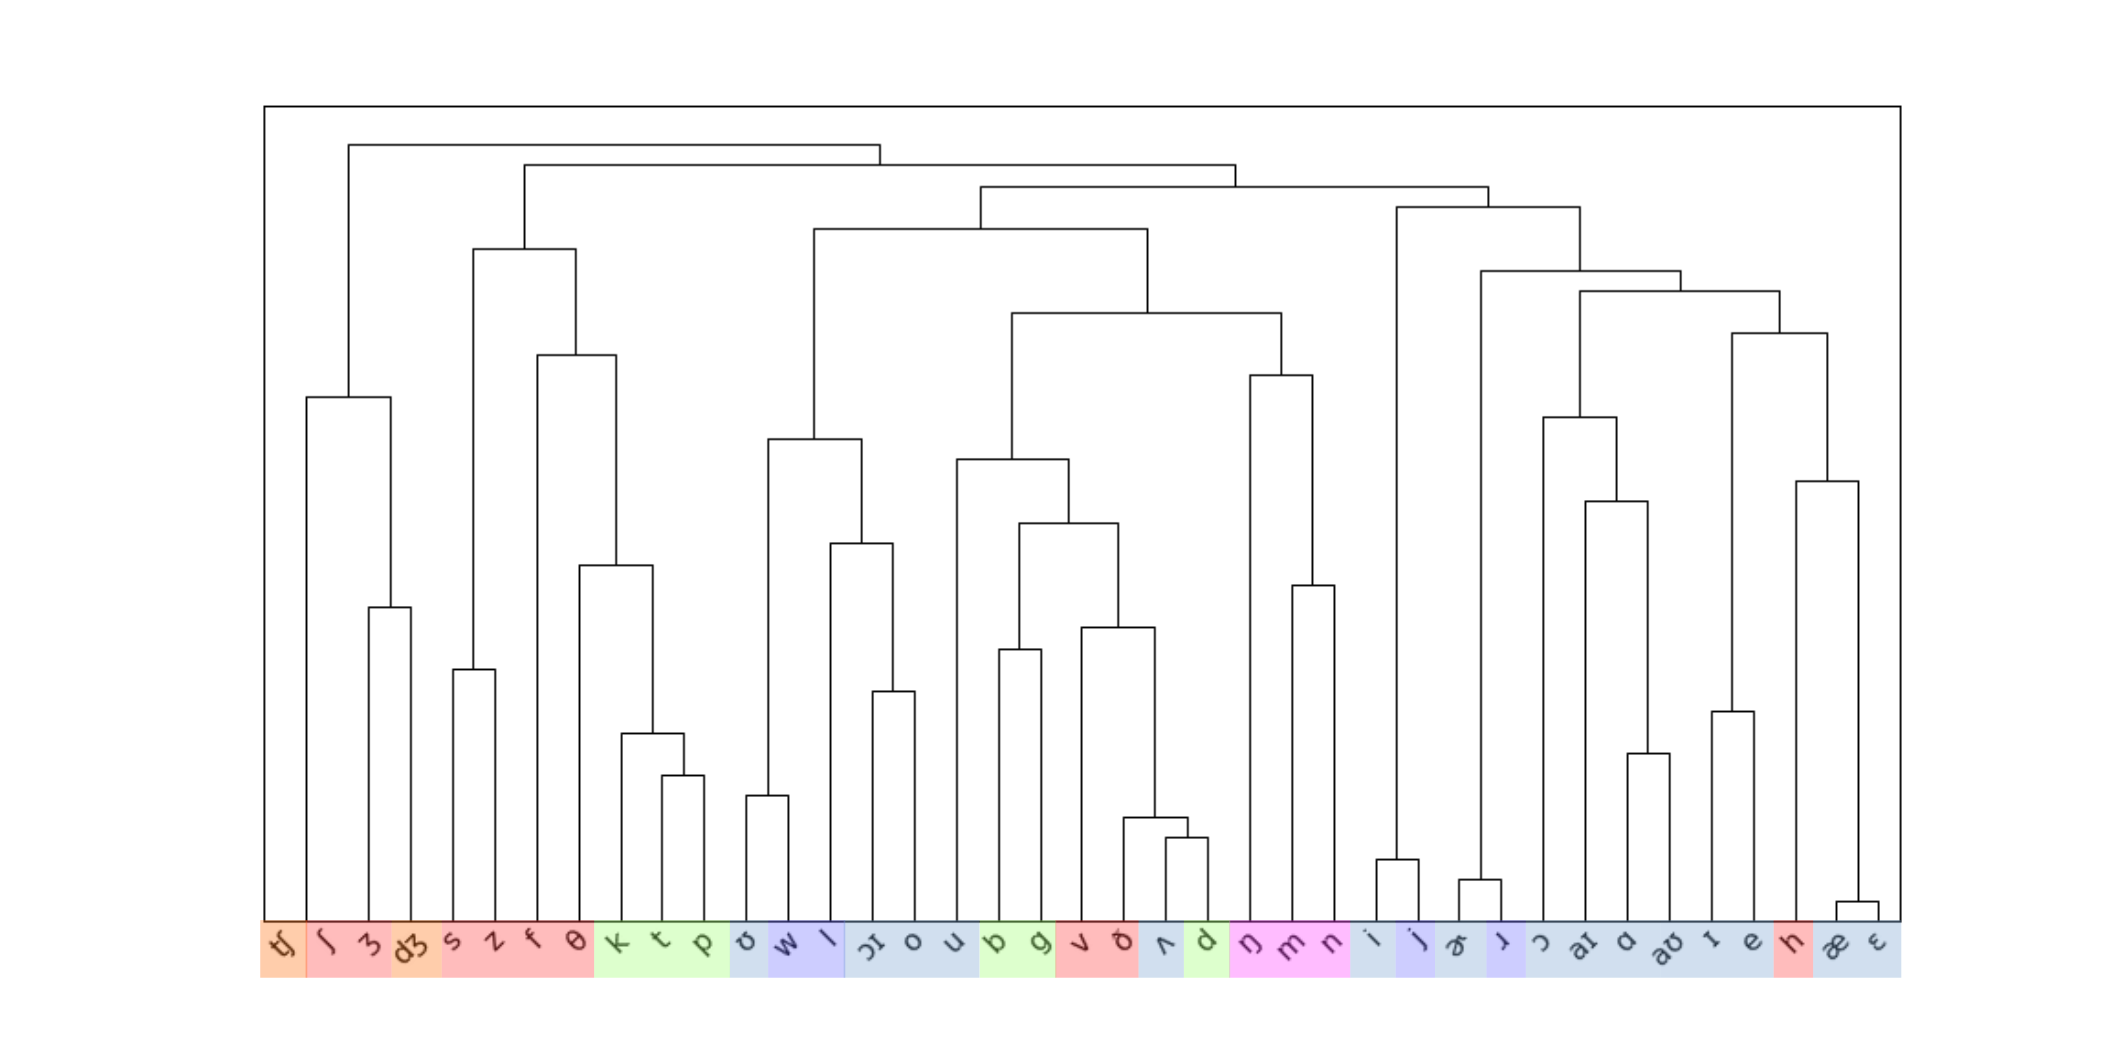
\includegraphics[scale=0.45]{figures/color-coded-activation0.png}
\caption{Hierarchical clustering of phoneme activation vectors on the first 
hidden layer.}
\label{fig:cluster-l0}
\end{figure*}




\subsection{Synonym discrimination}
\label{sec:synonym}

Next we simulate the task of distinguishing between pairs of synonyms, i.e.\ words with different acoustic forms but the same meaning. With a representation encoding phonological form, our expectation is that the task would be easy; in contrast, with a representation which is invariant to phonological form in order to encode meaning, the task would be hard. 

We generate a list of synonyms for each noun, verb and adjective in the validation data using Wordnet \citep{miller1995wordnet} synset membership as a criterion. Out of these generated word pairs, we select synonyms for the experiment based on the following criteria:
\begin{itemize}
\item both forms clearly are synonyms in the sense that one word can be replaced by the other without changing the meaning of a sentence,
\item both forms appear more than 20 times in the validation data, 
\item the words differ clearly in form (i.e. they are not simply variant spellings like {\it donut/doughnut, grey/gray}),
\item the more frequent form constitutes less than 95\% of the occurrences.
\end{itemize}
This gives us 2 verb, 2 adjective and 21 noun pairs.

For each synonym pair, we select the sentences in the validation set in which one of the two forms appears. We use the POS-tagging feature of NLTK \citep{bird2006nltk} to ensure that only those sentences are selected in which the word appears in the correct word category (e.g.\ {\it play} and {\it show} are synonyms when used as nouns, but not when used as verbs). We then generate spoken utterances in which the original word is replaced by its synonym, resulting in the same amount of utterances for both words of each synonym pair.

\begin{figure}[!ht]
  \centering
  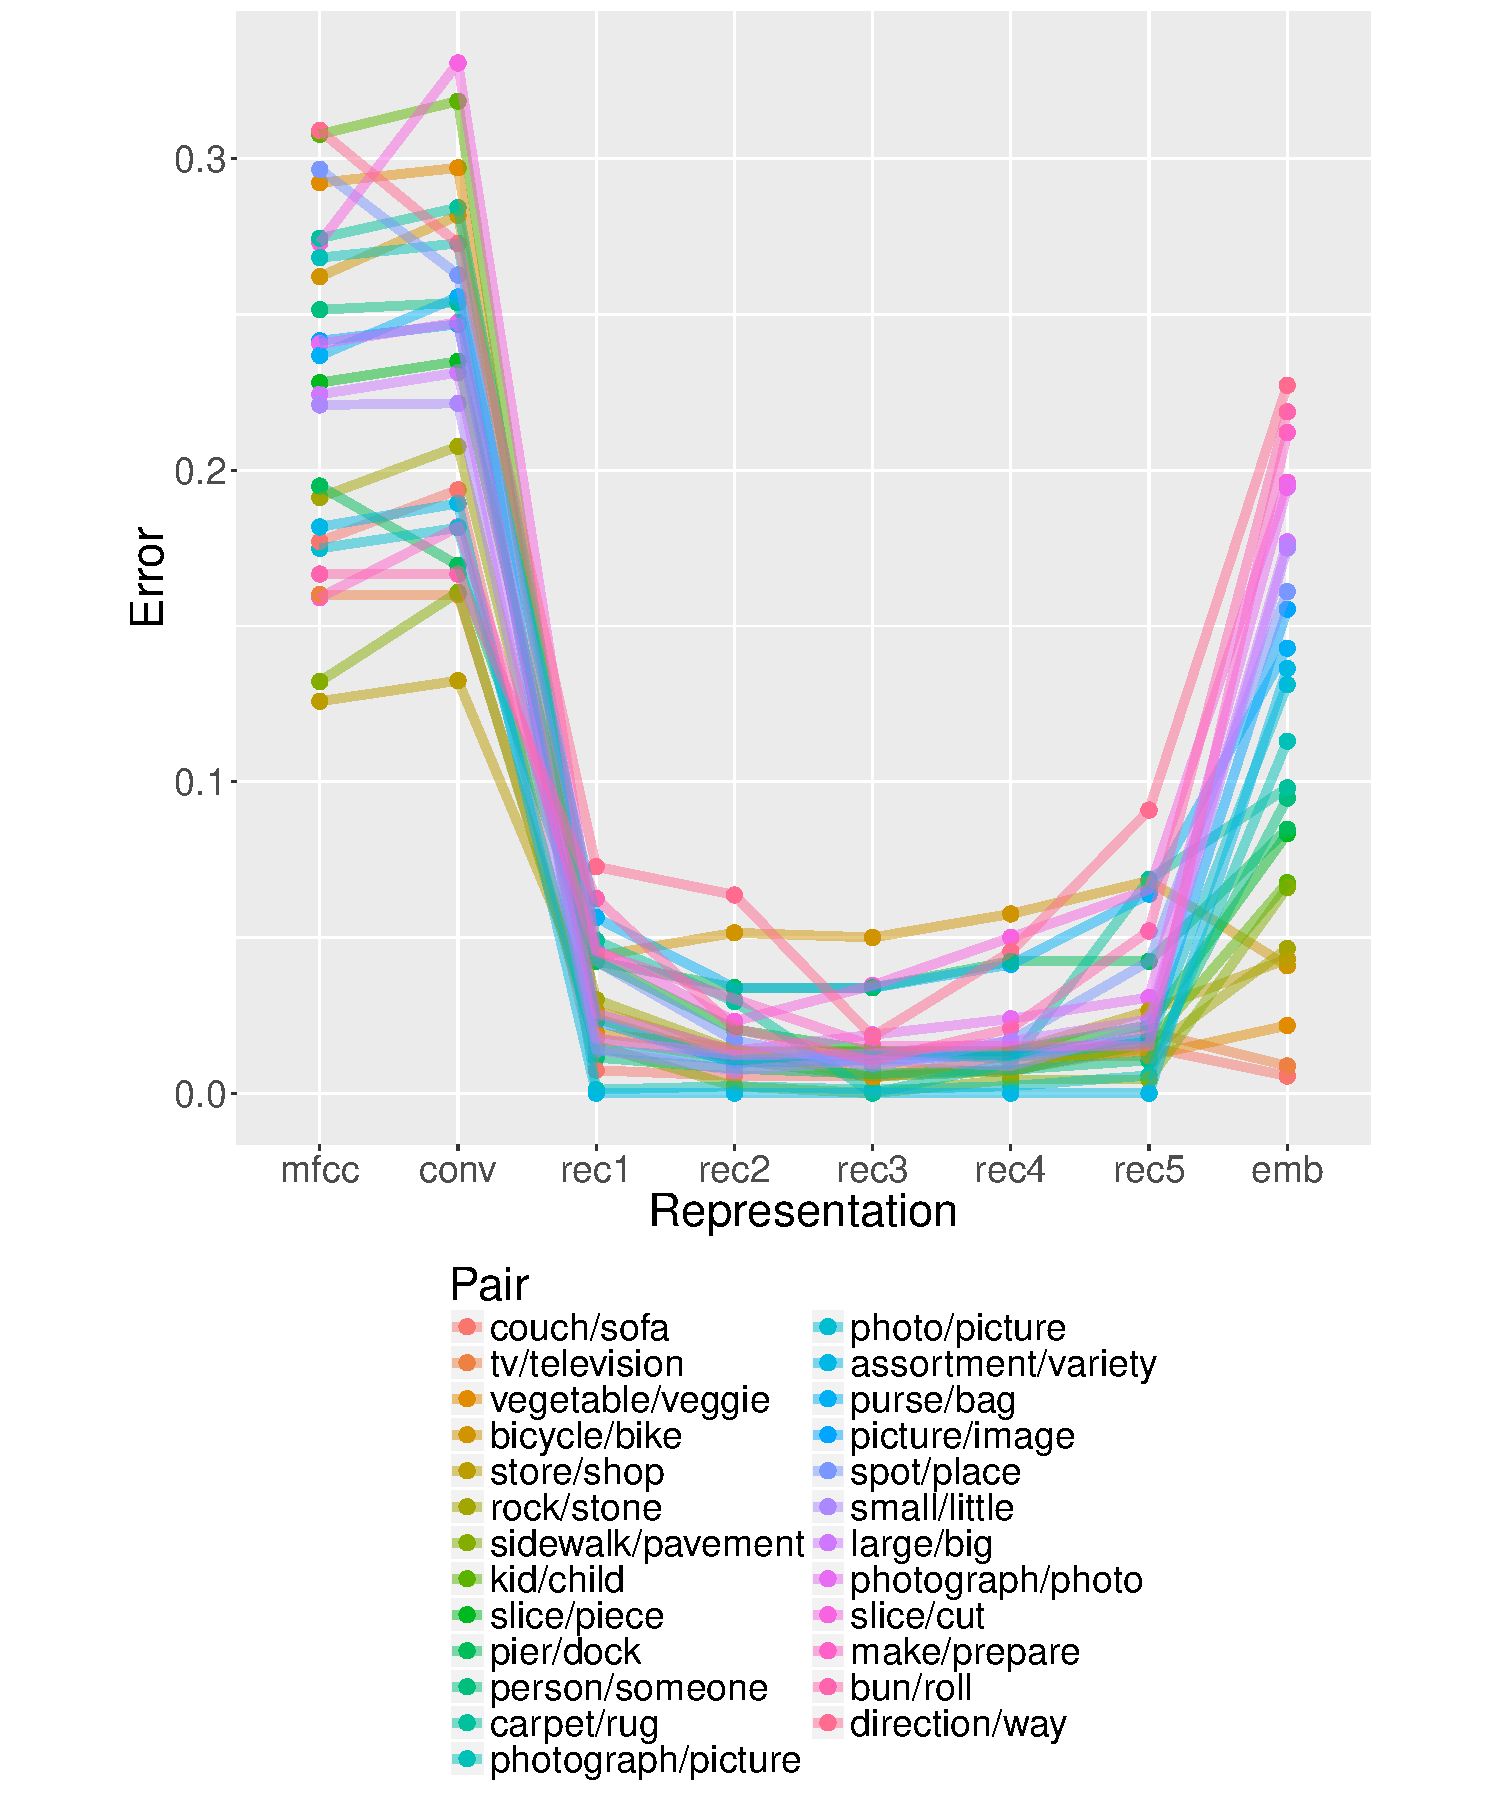
\includegraphics[scale=0.3]{figures/synonym.pdf}
  \caption{Synonym discrimination error rates, per representation and synonym pair.}
  \label{fig:synonyms}
\end{figure}


For each pair we generate a binary classification task using the MFCC features, the average activations in the convolutional layer, the average unit activations per recurrent layer, and the sentence embeddings as input features. For every type of input, we run 10-fold cross validation using Logistic Regression to predict which of the two words the utterance contains.  We used an average of 672 (minimum 96; maximum 2282) utterances for training the classifiers.

Figure~\ref{fig:synonyms} shows the error rate in this classification task for each layer and each synonym pair. Recurrent layer activations are more informative for this task than MFCC features or activations of the convolutional layer.  Across all the recurrent layers the error rate is small, showing that some form of phonological information is present throughout this part of the model. However, sentence embeddings give relatively high error rates suggesting that the attention layer acts to focus on semantic information and to filter out much of phonological form.



\section{Discussion}
\label{sec:conclusion}
Understanding distributed representations learned by neural networks
is important but has the reputation of being hard or even impossible. In
this work we focus on making progress on this problem for a particular
domain: representations of phonology in a multilayer recurrent neural network
trained on grounded speech signal. We believe it is important to
carry out multiple analyses using diverse methodology: any single
experiment may be misleading as it depends on analytical choices such
as the type of supervised model used for decoding, the algorithm used
for clustering, or the similarity metric for representational
similarity analysis. To the extent that more than one experiment
points to the same conclusion our confidence in the reliability of the
insights gained will be increased.

Earlier work \cite{chrupala2017representations} 
shows that encoding of semantics in our RNN model of grounded speech 
becomes stronger in higher layers, while encoding of form becomes weaker.
The main high-level results of our study confirm this pattern by showing that 
the representation of phonological knowledge is most accurate in the lower
layers of the model. This general pattern is to be expected as the
objective of the utterance encoder is to transform the input acoustic
features in such a way that it can be matched to its counterpart in a
completely separate modality. Many of the details of how this happens,
however, are far from obvious: perhaps most surprisingly we found that
a large amount of phonological information is still available up to the top
recurrent layer. Evidence for this pattern emerges from the phoneme
decoding task, the ABX task and the synonym discrimination task. The
last one also shows that the attention layer filters out and
significantly attenuates encoding of phonology and makes the utterance
embeddings much more invariant to synonymy.

Our model is trained on synthetic speech, which is easier to process than 
natural human-generated speech. While small-scale databases of natural 
speech and image are available \citep[e.g.\ the Flickr8k Audio Caption
Corpus,][]{harwath2015deep}, they are not large enough to reliably
train models such as ours. 
In future we would like to collect more data and apply our methodology to grounded 
human speech and investigate whether context and speaker-invariant phoneme 
representations can be learned from natural, noisy input. We would also like to make
comparisons to the results that emerge from similar analyses
applied to neuroimaging data.
  


\bibliographystyle{acl_natbib}
\bibliography{biblio}
\appendix


\end{document}
